%%%%%%%%%%%%%%%%%%%%%%%%%%%%%%%%%%%%%%%%%%%%%%%%%%%%%%%%%%%%%%%%%%%%%%%%%%%%%
%
% Vorlage für Seminararbeiten im Institut für Verteilte Systeme
% 
% HINWEISE
% 
%  1. Bei Nutzung für Seminarausarbeitungen darf insbesondere die Schriftart
%     und -größe nicht angepasst werden.
%  2. Die Vorlage unterstützt deutsche und englische Ausarbeitungen durch
%     Anpassung der babel Paketoptionen.
%  3. Folgende Angaben sollen angepasst werden:
%     - Titel der Arbeit
%     - Name und E-Mail-Adresse des Autors
%     - Titel des Seminars
%     - Semester
%  4. Die Vorlage sieht eine Lizensierung unter CC-BY-SA vor, die jedoch
%     nicht verpflichtend ist. Falls nicht gewünscht, bitte alle \thanks
%     Befehle auskommentieren.
%     Die gewählte Lizenz (CC-BY-SA) ist kompatibel mit einer möglichen
%     Veröffentlichung auf dem Volltextserver der Uni Ulm
%     (http://vts.uni-ulm.de).
%
%%%%%%%%%%%%%%%%%%%%%%%%%%%%%%%%%%%%%%%%%%%%%%%%%%%%%%%%%%%%%%%%%%%%%%%%%%%%%

% Based on the IEEE Journal style.
\documentclass[10pt,a4paper,compsoc,peer review papers]{IEEEtran}

\usepackage{graphicx}
\usepackage[cmex10]{amsmath}
\usepackage[ngerman]{babel} % Deutsche Ausarbeitung
% \usepackage[USenglish]{babel} % Englische Ausarbeitung
\usepackage{url}
\usepackage[colorlinks]{hyperref}
\usepackage{color}  % Definition von Linkfarben
\definecolor{DarkRed}{rgb}{0.5,0,0}
\hypersetup{
  colorlinks,
  citecolor=DarkRed,
  linkcolor=DarkRed,
  urlcolor=blue}
\usepackage[utf8]{inputenc}
\usepackage[T1]{fontenc}  % Korrekte Umlaute im Output

\newcommand\IEEEfirstsection[1]{%
  \noindent\raisebox{2\baselineskip}[0pt][0pt]%
  {\parbox{\columnwidth}{#1%
  \global\everypar=\everypar}}%
  \vspace{-1\baselineskip}\vspace{-\parskip}\par
}

\newcommand\cclicense{{\normalfont\sffamily\bfseries CC-BY-SA}}
\IfFileExists{ccicons.sty}{%
\usepackage{ccicons}
\renewcommand\cclicense{\ccbysa}
}

%% Eigene Einstellungen
\renewcommand{\arraystretch}{1.5}  % 1.5-facher Zeilenabstand in Tabellen

\begin{document}

\title{LEX 2016: Bestimmung der Wolkenhöhe und der Wasserdampfsäule mittels
Pyrgeometer}

\author{%
\IEEEauthorblockN{Lukas Kluft, Timorsha Rafiq-Dost}\\
\IEEEauthorblockA{\url{lukas.kluft@gmail.com}, \url{timorsha@live.de}}%
%
%\iflanguage{ngerman}{%
%\thanks{%
%\cclicense{}
%Diese Arbeit steht unter einer
%Creative Commons Namensnennung - Weitergabe unter gleichen Bedingungen
%3.0 Deutschland Lizenz.}%
%\thanks{\url{http://creativecommons.org/licenses/by-sa/3.0/de/}}%
%}{ % Englische Ausarbeitung
%\thanks{%
%\cclicense{}
%This work is licensed under a
%Creative Commons Attribution-ShareAlike 4.0 International License.}%
%\thanks{\url{http://creativecommons.org/licenses/by-sa/4.0/}}%
%}%
}

\IEEEpubid{\sffamily%
\makebox[\columnwidth]{\hfill Lehrexkursion Fehmarn}%
\makebox[\columnsep]{$\cdot$}%
\makebox[\columnwidth]{SS 2016,
Meteorologisches Institut - CEN, Universit"at Hamburg\hfill}}

\IEEEtitleabstractindextext{%
\begin{abstract}
Pyrgeometer messen die aus dem Halbraum eintreffende atmosphärische
Gegenstrahlung (5-50\,$\mu$m). Die Stärke der Gegenstrahlung hängt dabei vom
Zustand der Atmosphäre sowie der Bewölkung ab. Eine dichte Bewölkung kann
ebenso wie ein hoher Wasserdampfgehalt die langwellige Einstrahlung erhöhen. Im
Zuge der Lehrexkursion wurde untersucht, ob diese Zusammenhänge genutzt werden
können, um auf einfache Art und Weise meteorologische Zustandsgrößen
abzuleiten.
\end{abstract}%
}

\maketitle

\IEEEfirstsection{\section{Grundlagen}\label{sec:grundlagen}} Der Zustand der
Atmosphäre sowie die aktuelle Bewölkung haben einen starken Einfluss auf den
Strahlungshaushalt der Erde.  Wasserdampf in der Atmosphäre absorbiert
terrestrische Strahlung sehr effektiv.  Zusätzlich können Wasser- und
Eisteilchen in Wolken durch Streuung die Abstrahlung verringern.  Dadurch
verändern Wolken die optische Dicke der Atmosphäre.

Diese physikalischen Zusammenhänge legen nah, dass die langwellige
Einstrahlung Informationen über den Wassergehalt und die aktuelle Bewölkung
enthält.  Ziel ist es einerseits, über die Stärke der Einstrahlung eine
Abschätzung der Wolkenbasistemperatur vorzunehmen.  Unter zusätzlicher Annahme
eines Temperaturprofils kann so die Höhe der Wolkenunterkante abgeschätzt
werden. Des weiteren soll an wolkenfreien Tagen eine Aussage über den
integrierten Wasserdampfgehalt in der Atmosphäre getroffen werden.

\section{Motivation}
Wolken gehören zu den variabelsten und inhomogensten Bestandteilen der
Atmosphäre. Sie decken einen Größenbereich von einigen Metern, wie z.B
Cumuluswolken, bis zu mehreren hundert Kilometern (Frontensysteme) ab. Zudem
erstreckt sich auch die zeitliche Variabilität über mehrere Größenordnungen.
Von flachen Schönwettercumulus, dessen Lebenszeit mehrere Stunden beträgt, bis
zu mehreren Tagen bestehende Stratuswolken.

Die Existenz, Häufigkeit und die Art von Wolken im Allgemeinen sowie die
Wolkenhöhe im Speziellen spielen eine eminent große Rolle für das Wetter und
Klima. Neben Niederschlagsprozessen beeinflussen sie auch die Strahlungsbilanz
der Erde. Die auf die Erde einfallende Solarstrahlung wird über Wolken und
Atmosphäre teilweise in das Weltall zurückgeworfen, weshalb einige Wolkentypen
zu Abkühlung des Planeten tendieren. Die abgegebene terrestrische Strahlung vom
Erdboden, welche in Richtung Himmel gerichtet ist, wird von Wolken absorbiert.
Die dadurch bereitgestellte Energie kann genutzt werden, um langwellige
Strahlung in Richtung Erdoberfläche zurück zu emittieren. Wolken haben 
dementsprechend auch einen erwärmenden Effekt auf die Erde und sind
ausschlaggebend für den Treibhauseffekt (IPCC, 2013 \cite{ipcc2013}).
Ob eine Wolke erwärmend oder abkühlend auf die Atmosphäre wirkt hängt
entscheidend von der Albedo, der optischen Dicke und der thermischen
Ausstrahlung, also der Wolkenhöhe ab.

Außerdem hat die Wolkenunterkante auch praktische Bedeutung, wie zum Beispiel
in der Luftfahrtberatung. Bei Sichtflugbedingungen etwa darf eine gewisse
Wolkenuntergrenze nicht unterschritten werden.

Hinsichtlich der Wichtigkeit der Wolkenhöhe wurden im Rahmen der Lehrexkursion
(LEX) auf Fehmarn Strahlungsmessungen mit einem Pyrgeometer durchgeführt.
Pyrgeometer messen dabei die aus dem Halbraum eintreffende atmosphärische
Gegenstrahlung in einem Wellenlängenbereich zwischen 5\,$\mu$m und 50\,$\mu$m.
Die Grundidee und Motivation dieses Versuches liegt darin, das
Leistungspotenzial und die Fähigkeiten eines einfachen Messinstruments wie
einem Pyrgeometer zu testen. Die langwellige Einstrahlung und die Temperatur,
welche mittels Pyrgeometer beziehungsweise einem Thermometer ermittelt werden,
sind jene Messgrößen, die für diesen speziellen Versuch von Bedeutung sind. Es
soll geklärt werden, inwiefern und mit welcher Genauigkeit es möglich ist,
atmosphärische Zustandsgrößen aus diesen einfachen Messgrößen abzuleiten.

Im Folgenden werden dafür zunächst der zugrunde liegende Messaufbau vorgestellt
(Abschnitt~\ref{sec:aufbau}). Abschnitt~\ref{sec:datensatz} erläutert
den über die Messperiode gewonnen Datensatz. Darauf folgend werden die
Ergebnisse des Projekts präsentiert. Die Konzentration liegt einerseits in der
Ermittlung der Wolkenbasishöhe (Abschnitt~\ref{sec:wolkenhoehe}) sowie in der
Bestimmung des integrierten Wasserdampfgehalts der Atmosphäre
(Abschnitt~\ref{sec:wasserdampfsäule}). Abschließend folgen in
Abschnitt~\ref{sec:schlussfolgerungen} und \ref{sec:ausblick} ein Fazit sowie
ein kurzer Ausblick.

Eine Sammlung der verwendeten Skripte zur Durchführung der 
Strahlungstransfersimulationen sowie der anschließenden Auswertung findet sich 
frei zugänglich auf GitHub\footnote{\url{https://github.com/lkluft/cloud-base}}.

\section{Messaufbau}\label{sec:aufbau}

\begin{figure}[ht]
  \centering
  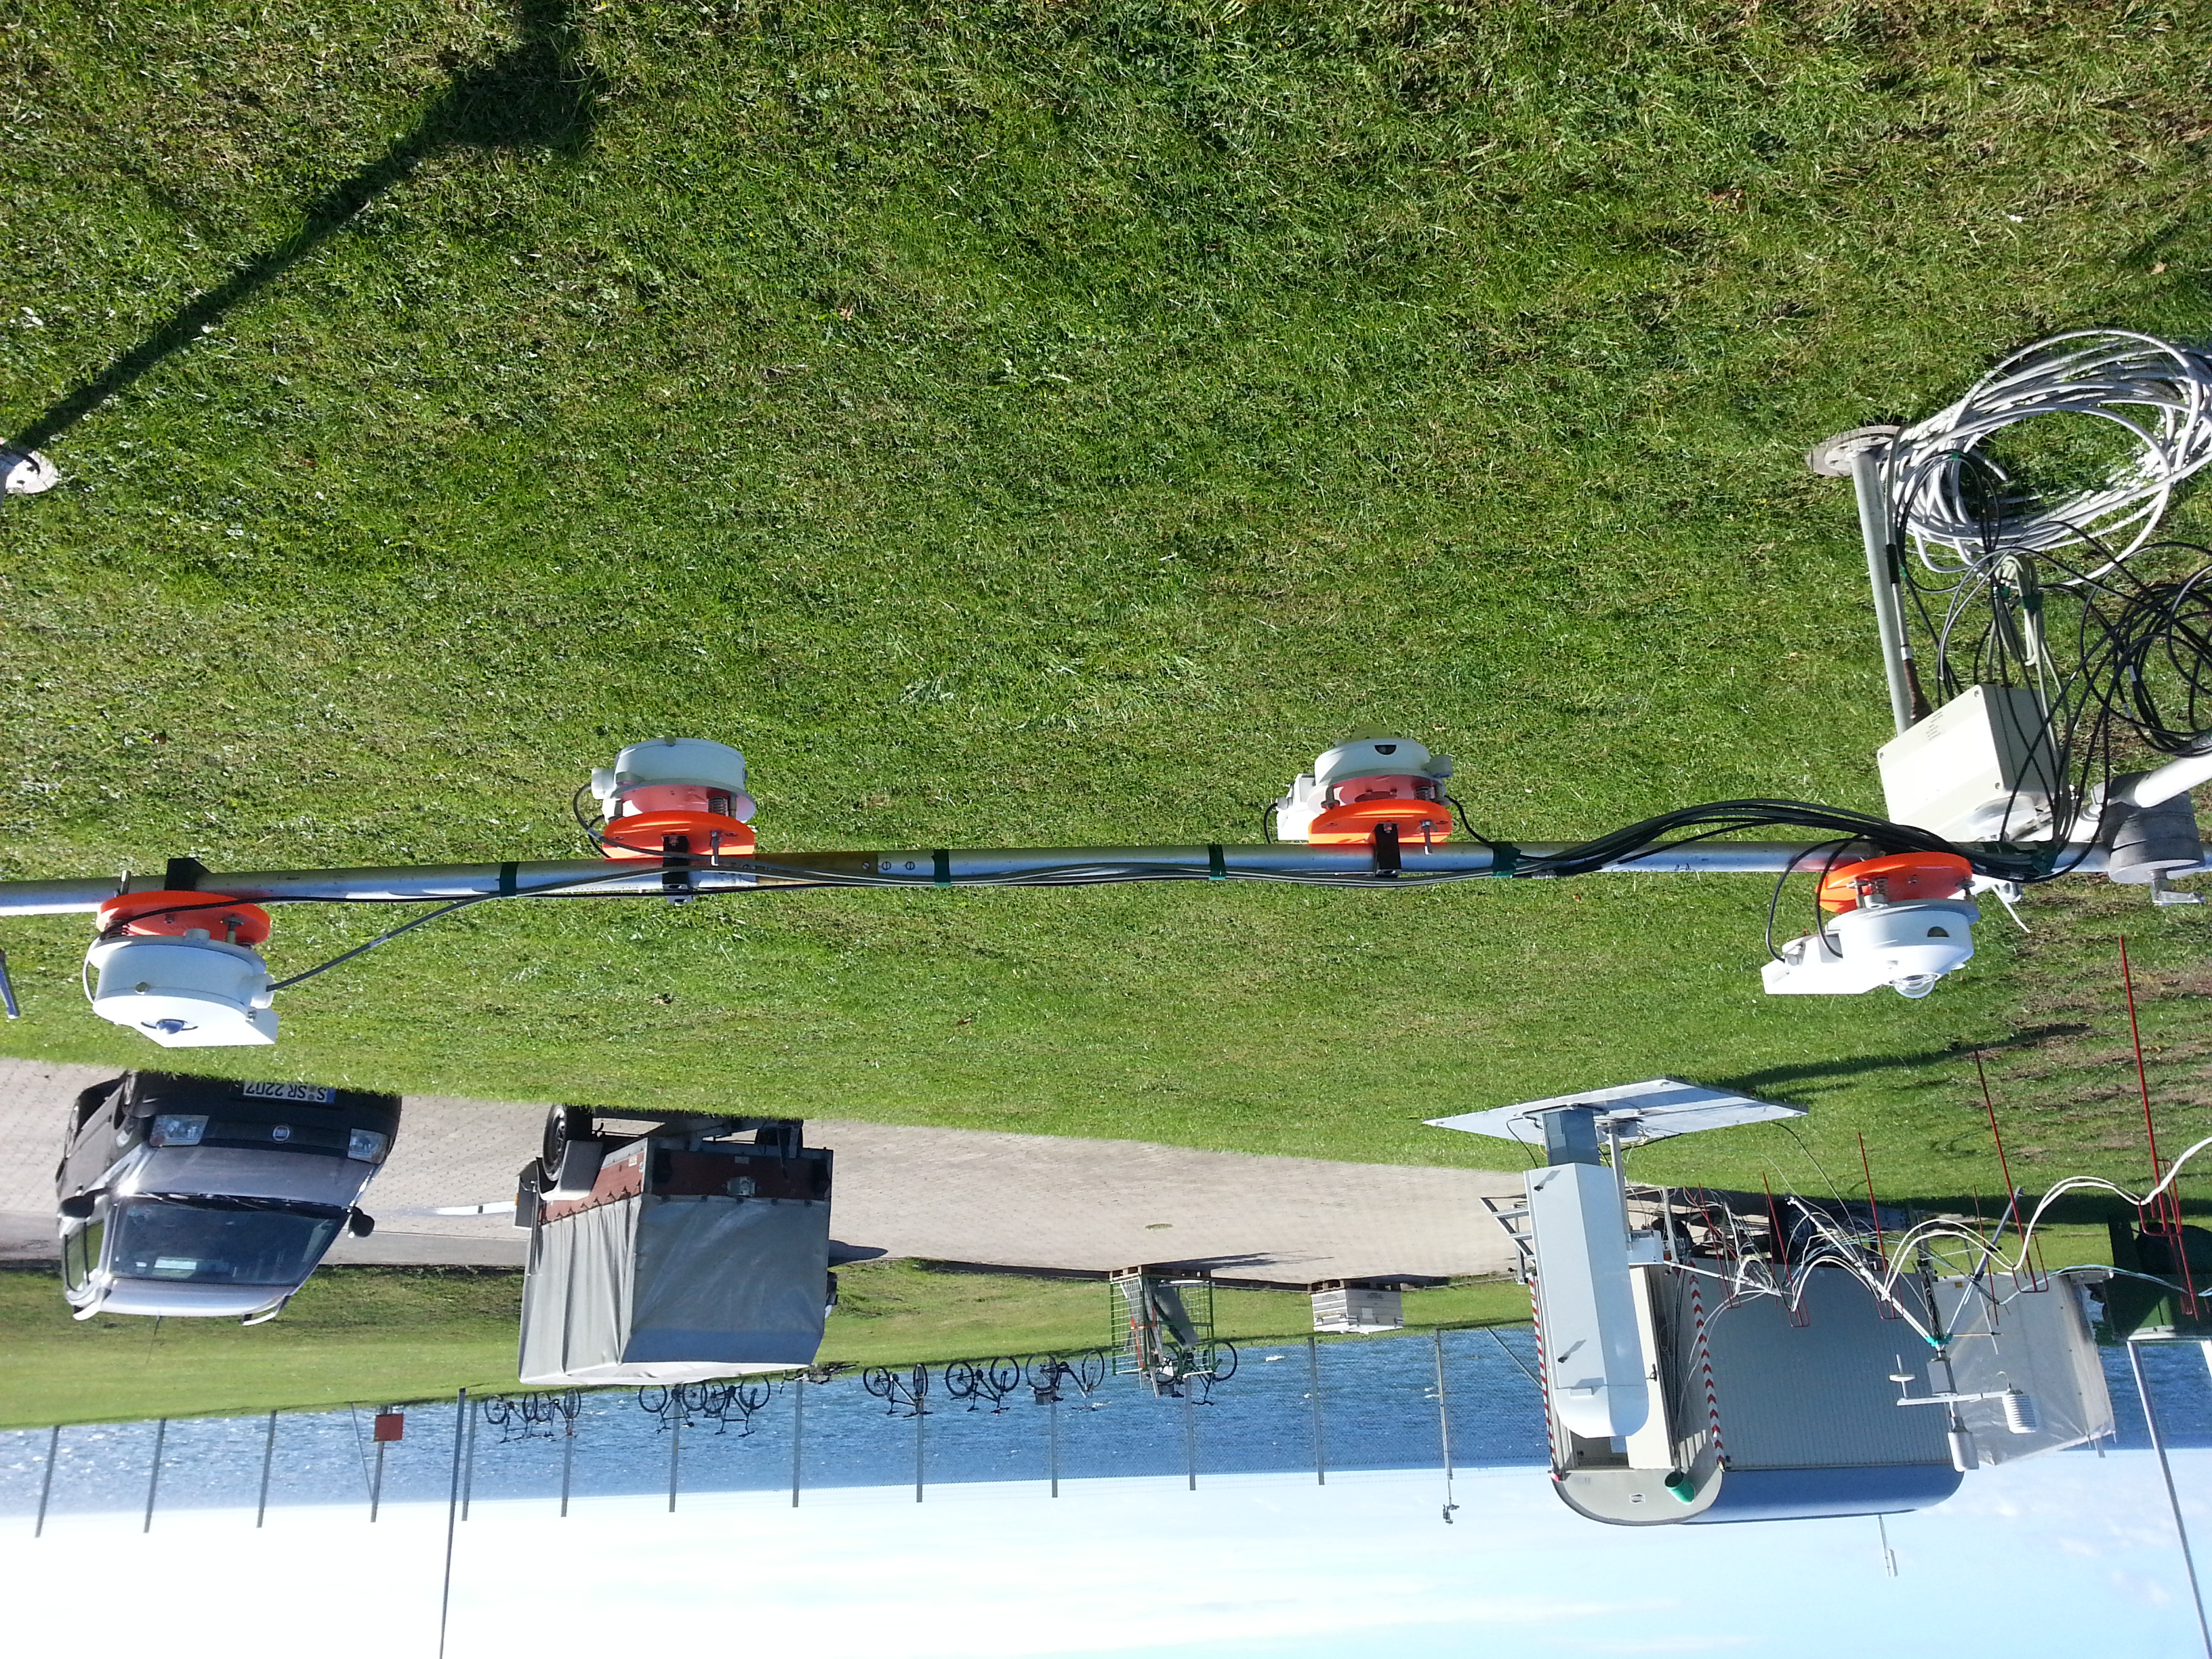
\includegraphics[angle=180,width=0.45\textwidth]{figures/aufbau.jpg}
  \caption{Aufbau des Strahlungsgartens.}
  \label{fig:aufbau}
\end{figure}

Für die Messung der Strahlung wurde eine Strahlungsstation (Strahlungsgarten)
auf einer Wiese installiert. Der genaue Messaufbau des Strahlungsgartens kann
der Abbildung~\ref{fig:aufbau} entnommen werden. Auf der Wiese wird
die Ein- und Ausstrahlung sowohl in langwelligen als auch kurzwelligen Teil
des Frequenzspektrumgs gemessen. Für die langwellige Strahlung aus dem oberen
und unteren Halbraum werden Pyrgeometer und für die kurzwellige Strahlung
Pyranometer verwendet. Die Instrumente befinden sich etwa einen Meter über der
Erdoberfläche. Zusätzlich dazu wurde in unmittelbarer Nähe ein Schattenring
aufgestellt, um den diffusen Anteil der kurzwelligen Einstrahlung zu bestimmen.
Die exakten geographischen Positionen des Schattenringes sowie des
Strahlungsgartens können der Tabelle~\ref{tab:gps} entnommen werden.

\begin{table}[ht]
  \centering
  \caption{GPS-Koordinaten des Strahlungsgartens und des Schattenrings.}
  \label{tab:gps}
  \begin{tabular}{l|l|l}
    \textbf{Geräte}        & \textbf{Koordinaten Nord} & \textbf{Koordinaten Ost} \\\hline
    Schattenring           & N\,54$^\circ$ 29.677' & E\,11$^\circ$ 14.414' \\
    Strahlungsgarten Nord  & N\,54$^\circ$ 29.679' & E\,11$^\circ$ 14.425' \\
    Strahlungsgarten Mitte & N\,54$^\circ$ 29.678' & E\,11$^\circ$ 14.427' \\
    Strahlungsgarten Süd   & N\,54$^\circ$ 29.676' & E\,11$^\circ$ 14.425' \\
  \end{tabular}
\end{table}

Zusätzlich wurden ein Ceilometer von VAISALA und das Mikrowellenradiometer
HATPRO als Referenz genutzt, um die aus den Messungen des Pyrgeoemters
abgeleiteten Ergebnisse vergleichen zu können. Das Ceilometer und Radiometer
sind ebenfalls auf der Wiese in unmittelbarer Nähe zum Strahlungsgarten
betrieben wurden. Das Ceilometer sendet Laserimpulse aus. Diese werden von 
Wolken und Staubpartikeln zurückgestreut. Das zurückgestreute Laserlicht wird im 
Messgerät detektiert.  Aus der Laufzeit der Signale und der Lichtgeschwindigkeit 
wird die Entfernung zum Ort der Streuung berechnet. Somit lässt sich die Höhe
der Wolkenunterkante hochauflösend bestimmen.

Das  HATPRO misst die thermische Ausstrahlung der Atmosphäre. Durch eine
entsprechende Auswahl der Empfangsfrequenzen kann die Emission von
Mikrowellenstrahlung bestimmter Spurengase, von Flüssigwasser sowie von
Eiskristallen empfangen werden. So befindet sich beispielsweise bei Frequenzen
von 20 bis 30\,GHz ein schwaches Absorptionsband von Wasserdampf. Messungen der
Strahlungstemperatur an der Flanke dieses Absorptionsbandes erlaubt eine
Abschätzung des Gesamtwasserdampfgehalts (Integrated Water Vapour $IWV$), sowie
eine Abschätzung des Wasserdampfprofiles (jedoch in geringer vertikaler
Auflösung). Die aufgenommenen Wolkenbasishöhen und der IWV vom 
Ceilometer bzw.\ HATPRO dienen im folgenden als Referenzdaten.

Das Messgelände ist durch diverse Besonderheiten gekennzeichnet: In
südlicher Richtung vom Messaufbau befindet sich ein Funkturm. Außerdem befindet
sich der Aufbau in direkter Küstennähe. Bei tiefstehender Sonne kann es zu
Einfluss durch Reflexionen auf der Wasseroberfläche kommen. Der Einfluss auf
die Messung ist wahrscheinlich jedoch sehr gering, da die verwendeten Instrumente
nah am Horizont nicht sensitiv sind.

\section{Datensatz}\label{sec:datensatz}
Die Lehrexkursion fand in dem Zeitraum vom 29. August bis 9. September 2016
statt. Jedoch stehen die Daten nicht für den kompletten Zeitraum zur Verfügung.
Der letzte Tag wurden genutzt um die Geräte abzubauen, daher können
ausschließlich die Daten vom 19.08. bis zum 07.09.2016 berücksichtigt werden.
Es ist darauf hinzuweisen, dass ein 15-minütiger Stromausfall am 01.09.2016
von 14.20 UTC bis 14.35 UTC dafür gesorgt hatte, dass auch hier keine Daten
verfügbar sind.

Die Messungen des Pyrgeometers und Ceilometers sind resistent gegenüber
Wettereinwirkungen wie Regen, sodass permanent verwertbare Daten von der
atmosphärischen Gegenstrahlung bzw. Wolkenunterkantenhöhe geliefert werden
konnten. Beide Geräte liefern Daten in einminütiger Auflösung. Die Messungen
des Radiometers liegen in zehnminütiger Auflösung vor. Beim HATPRO gibt es
allerdings Einschränkungen, sobald es regnet; während Regen-Events sind die
$IWV$-Messdaten unbrauchbar.

\section{Strahlungstransfer}\label{sec:strahlungstransfer}
\subsection{Grundlagen}\label{subsec:grundlagen}
Pyrgeometer messen den gesamten Strahlungsfluss im langwelligen Bereich des
Frequenzspektrums. Um genauere Informationen darüber zu gewinnen, aus welchen
Teilen der Atmosphäre die gemessene Strahlung stammt, wurden
Strahlungstransferrechnungen durchgeführt.

Für die Berechnung wurde der Atmospheric Radiative Transfer Simulator (ARTS)
verwendet \cite{Eriksson2011}. ARTS ist ein physikalisches
Strahlungstransfermodell für den Millimeter- und Submillimeterbereich des
elektromagnetischen Strahlungsspektrums.

Bei der Simulation von Strahlungsflüssen ist eine genaue Kenntnis des
Atmosphärenzustands erforderlich.  Dieser wird benötigt, um die
Strahlungseigenschaften der Atmosphäre zu bestimmen. Die hier betrachteten
Vorgänge sind vom Verhalten des Wasserdampfes dominiert. Aus diesem Grund wird
Streuung vernachlässigt und lediglich Absorption durch die Atmosphäre
berücksichtigt.  Wie stark ein Gas absorbiert hängt auch von der Frequenz der
betrachteten Strahlung ab. In Linienkatalogen lassen sich Informationen über
die Position und Stärke von Absoprtionslinien finden. Für die durchgeführten
Rechnungen wurde der HiTran-Katalog in der Version von 2012 verwendet
\cite{Rothman2013}.  Abbildung~\ref{fig:opacity} zeigt die optische Dicke für
verschiedene Absorber und Frequenzen des elektromagnetischen Spektrums.
Die optische Dicke $\tau$ ist das Wegintegral über den Absorptionskoeffizienten
$\alpha$ (Gleichung~\ref{eq:tau}) und erlaubt somit eine Aussage über die
Gesamtabsorption in der Luftsäule.
\begin{equation}\label{eq:tau}
\tau(0,\,z) = \int_0^z \alpha(s)\,\partial s
\end{equation}
Es ist klar zu erkennen, dass Wasserdampf nahezu im gesamten betrachteten
Frequenzbereich der dominante Absorber ist. Lediglich um 20\,THz befinden sich
einige $CO_2$ Linien. Auch wenn die weiteren Absorber insgesamt nur einen
kleinen Anteil an der Gesamtabsorption der Atmosphäre haben, müssen sie für
eine akkurate Simulation des Strahlungsflusses berücksichtigt werden.

\begin{figure}[ht]
  \centering
  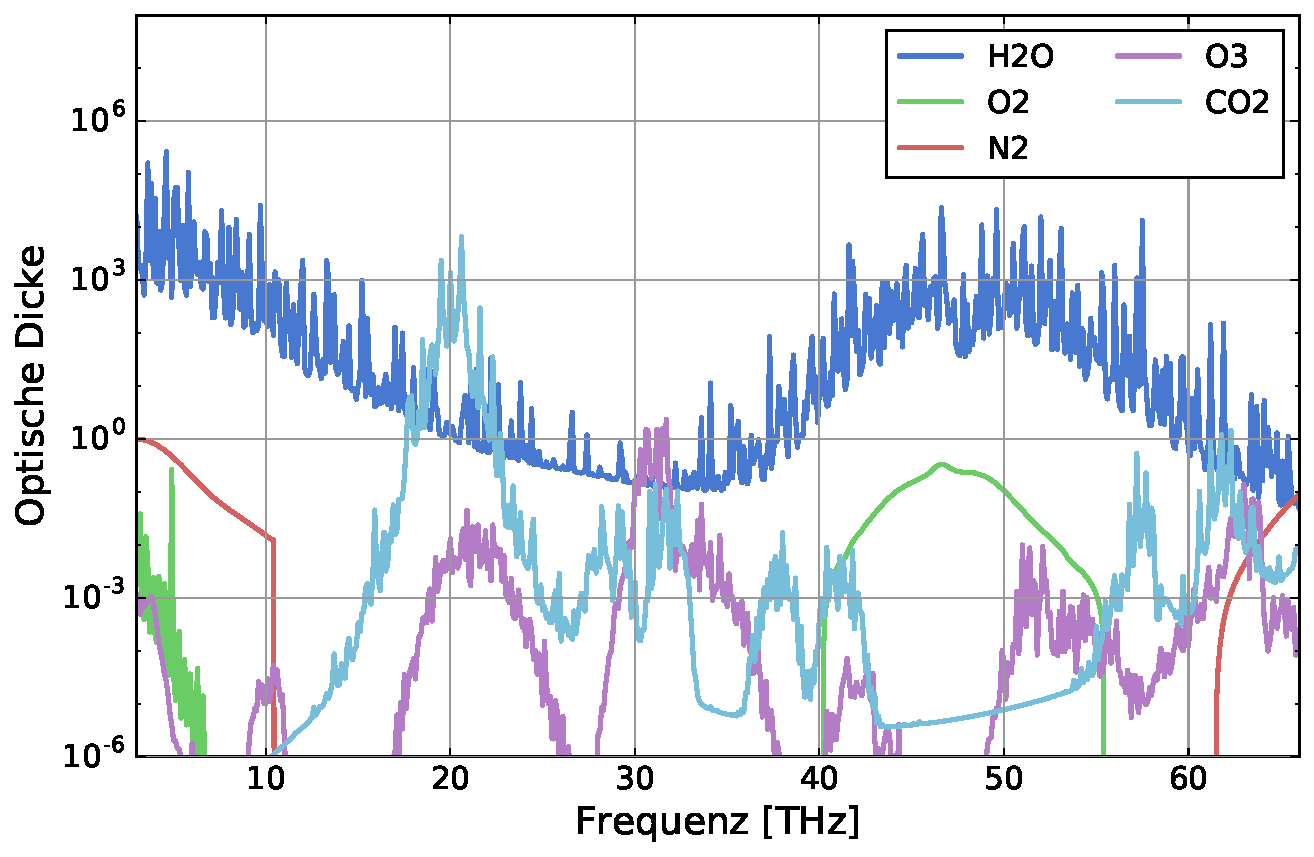
\includegraphics[width=0.5\textwidth]{figures/midlatitude-summer_opacity.pdf}
  \caption{Frequenzabhängigkeit der optischen Dicke~$\tau$ für verschiedene
  Absorber.}
  \label{fig:opacity}
\end{figure}

Der Zustand der Atmosphäre kann auf verschiedene Arten beschrieben werden.
Strahlungstransfersimulationen können auf Radiosonden, Klimatologien,
oder Modellergebnissen basieren. Um einen Überblick über den Strahlungsfluss im
langwelligen Frequezbereich zu erlangen, wurde eine eine Klimatologie aus dem
Satz der FASCOD Atmosphären verwendet \cite{Anderson1986}. Diese Klimatologien
beschreiben Temperatur, Druck und Zusammensetzung der Atmosphäre auf 46
vertikalen Schichten. Um die atmosphärischen Verhältnisse während der
Lehrexkursion möglichst gut abzubilden, wurde eine Klimatologie für den Sommer
in den mittleren Breiten verwendet.

Zur Untersuchung der Abängigkeit der langwelligen Einstrahlung von der
Wasserdampfsäule wird ein möglichst großer Datensatz benötigt. Dieser erlaubt
es statistische Zusammenhänge sicherer zu erfassen. Der Atmosphärensatz von
Chevallier \cite{Chevallier2006} umfasst 25.000 Atmosphären, die dem globalen
Zirkulationsmodell des europäischen Zentrum Zentrum für mittelfristige
Wettervorhersage (EZMW) entstammen. Der Datensatz wurde so
zusammengestellt, dass er ein breites Feld möglicher atmosphärischer Zustände
abbildet. Extrema sind hierbei deutlich überrepräsentiert. Dies ist bewusst
gewählt und erleichtert Regressionen, da in einem weiten Wertebereich
eine hohe Datendichte gewährleistet ist.

\subsection{Simulation des Pyrgeometers}\label{subsec:simulation_pyrgeometer}
Pyrgeometer messen den langwelligen Strahlungsfluss im gesamten Halbraum. Der
Strahlungstransfer muss daher nicht nur für eine große Anzahl von Frequenzen,
sondern zusätzlich für verschiedene Einfallswinkel berechnet werden. Diese
Ergebnisse können dann spektral und räumlich integriert werden, um eine
Abschätzung der atmosphärischen Gegenstrahlung zu ermöglichen.

\begin{figure}[ht]
  \centering
  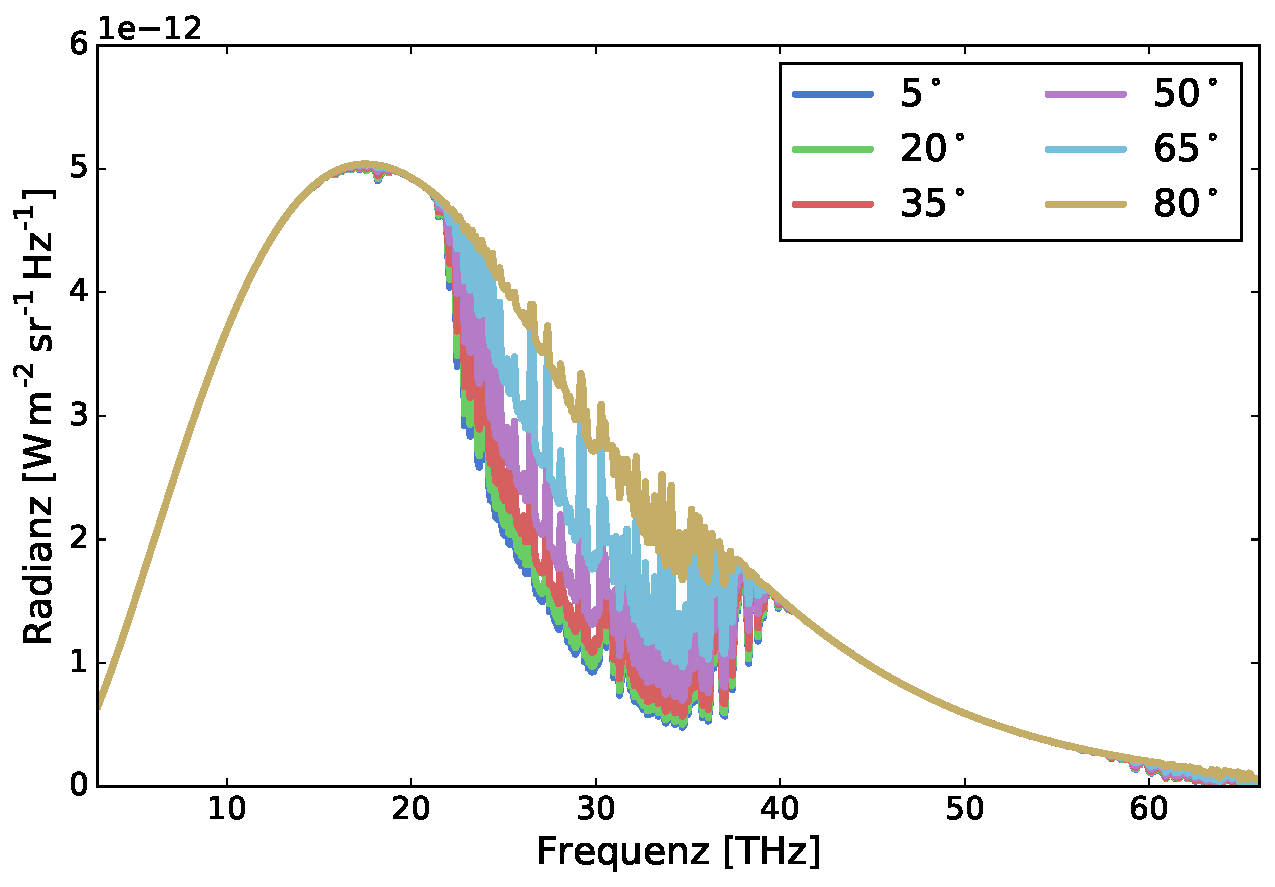
\includegraphics[width=0.5\textwidth]{figures/lwr_spectrum_elevation.pdf}
  \caption{Frequenzspektrum für verschiedene Einfallswinkel.}
  \label{fig:spectrum_elevation}
\end{figure}

Die Intensität der einfallenden atmosphärischen Gegenstrahlung ist stark vom
Beobachtungswinkel abhängig. Bei Betrachtungen nahe dem Zenith ist der optische
Weg durch die Atmosphäre sehr kurz. Dies verringert auch die optische Dicke der
Atmosphäre, wodurch Strahlung aus höheren Atmsphärenschichten den Boden
erreichen kann. Nahe dem Horizton ist der Weg durch die Atmosphäre weiter.
Zusätzlich ist die Wasserdampfkonzentration in der Troposphäre deutlich höher
als in oberen Atmosphärenschichten. Beides führt dazu, dass die optische Dicke
bei flachem Einfallswinkel stark zunimmt und fast ausschließlich
Strahlungssignale aus der nahen Umgebung gemessen werden.
Abbildung~\ref{fig:spectrum_elevation} zeigt das Intensitätsspektrum für
diverse Einfallswinkel. Es ist zu erkennen, dass Strahlung aus Einfallswinkeln
knapp über dem Horizont ($5^\circ$) eine höhere Intensität hat als solche, die
senkrecht einfällt. Dies ist direkte Folge der Temperature der emittierenden
Atmosphärenschichten nahe dem Boden.

Bei der räumlichen Integration der Strahlungsflüsse muss die Abängigkeit vom
Einfallswinkel $\theta$ deshalb genau bedacht werden. Zum einen wird nur der
senkrecht zur Oberfläche einfallenden Anteil der Strahlung berücksichtigt
($\cos\theta$). Strahlung nahe dem Zenith wird somit stärker gewichtet als
solche am Horizont. Strahlung nahe dem Horizont nimmt jedoch einen deutlich
großeren Raumwinkel ein ($2\pi\sin\theta$). Beide Effekte werden bei der
Integration (Gleichung~\ref{eq:lwr_integral}) der Strahlungsflüsse aus der
Strahlungstransfersimulation berücksichtigt.

\begin{equation}\label{eq:lwr_integral}
    L = \int 2\pi \sin\theta \cdot \cos\theta \cdot I_\theta \,\partial\theta
\end{equation}

Es lässt sich somit zusammenfassen, dass die Simulation der Messungen eines
Pyrgeometers einen erheblichen Aufwand darstellt. Der Strahlungsrtransfer muss
nicht nur für sehr viele Frequenzen, sondern auch für diverse Einfallswinkel
durchgeführt werden. Für einzelne atmosphärische Profile lässt sich diese
Rechnung in kurzer Zeit durchführen. Sollen jedoch etliche Atmosphären
prozessiert werden (Kapitel~\ref{sec:wasserdampfsäule}) muss das Verfahren
optimiert werden. ARTS bietet hierzu die Möglichkeit sogenannter
\textit{lookup table}. Diese Tabellen werden einmalig im Vorfeld berechnet
und enthalten Informationen über die Absorption bei verschiedensten
atmosphärischen Zuständen. In späteren Strahlungstransfersimulationen werden
diese Paramter dann nicht mehr explizit berechnet, sondern die
Absorptionskoeffizienten werden aus den vorberechneten Tabellenwerten
interpoliert. Auf diese Weise ist es möglich, auch mehrere tausend
Atmospärenprofile in annnehmbarer Zeit zu simulieren.

\section{Wolkenhöhe}\label{sec:wolkenhoehe}
Im ersten Teil der Untersuchungen wurde versucht die Wolkenbasishöhe mittels
Messungen der langwelligen Einstrahlung $L$ sowie der bodennahen Temperatur
zu ermitteln.

Das Prinzip hinter diesem Verfahren liegt darin, dass niedrige Wolken eine
höhere Temperatur als hohe Wolken haben. Dieser Temperaturunterschied ist als
Signal in der langwelligen Einstrahlung zu erkennen
(Abschnitt~\ref{subsec:clb_prinzip}). Die Ergebnisse der durchgeführten
Falluntersuchung sind in Abschnitt~\ref{subsec:clb_ergebnisse} dokumentiert.

\subsection{Messprinzip}\label{subsec:clb_prinzip}

\begin{figure}[ht]
  \centering
  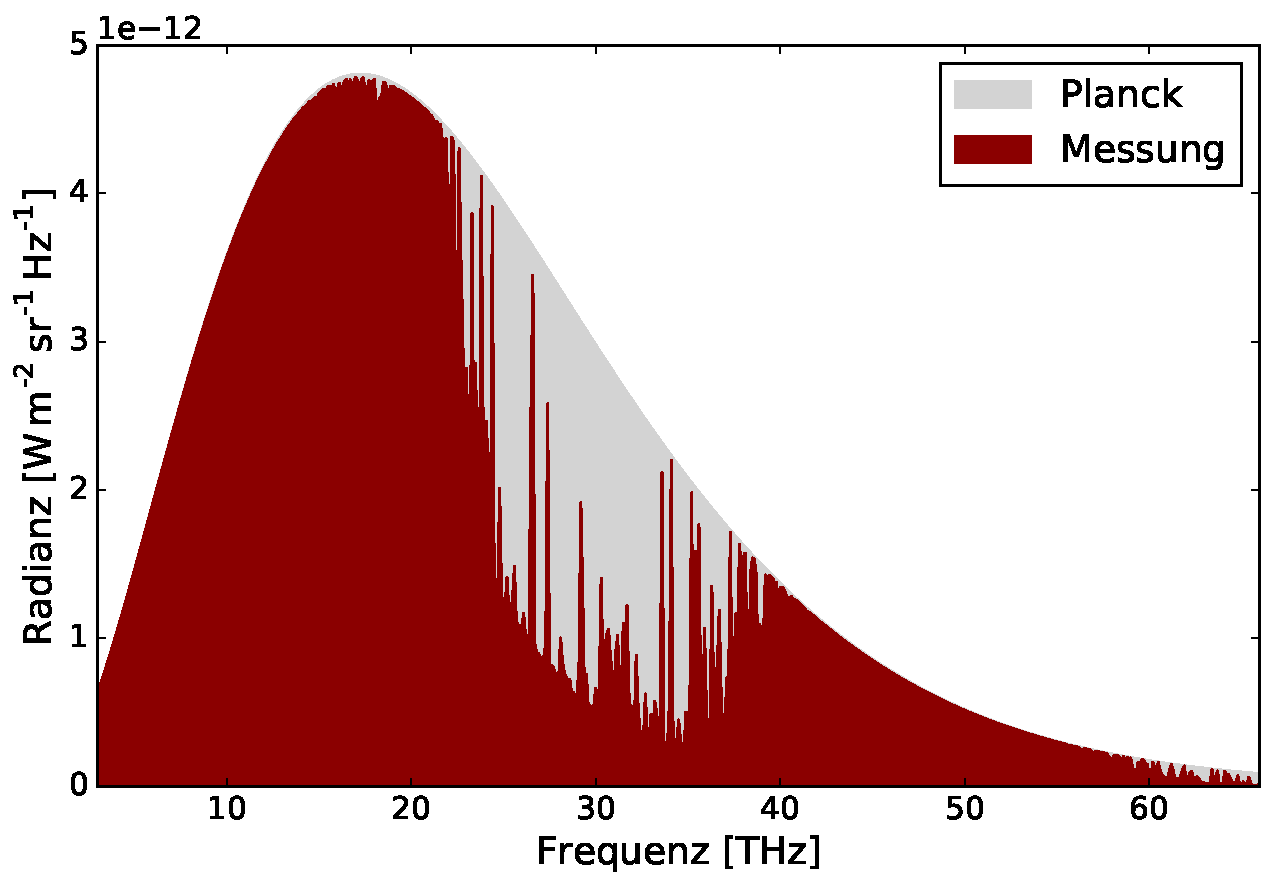
\includegraphics[width=0.5\textwidth]{figures/midlatitude-summer_spectrum.pdf}
  \caption{Simuliertes Spektrum der langwelligen Einstrahlung im Vergleich zur
  Planckkurve bei 2\,m-Temperatur.}
  \label{fig:lwr_spectrum}
\end{figure}

Das Messprinzip beruht auf der Annahme, dass die Messung des Pyrgeometers eine
Information über die Temperatur der Wolkenunterkante beinhaltet. Um diese
grundlegende Annahme zu überprüfen, wurden Strahlungstransfersimulationen
durchgeführt (Abschnitt~\ref{sec:strahlungstransfer}).
Abbildung~\ref{fig:lwr_spectrum} zeigt ein Frequenzspektrum, welches aus diesen
Simulationen resultiert. Dargestellt ist die simulierte langwellige
Einstrahlung für eine Klimatologie, die den Sommer in den mittleren Breiten
repräsentiert.  Zusätzlich wurde die Planckkurve bei bodennaher Temperatur
eingefügt. In weiten Bereichen des elektromagnetischen Spektrums verlaufen
simulierte Einstrahlung und Planckkurve deckungsgleich, was bedeutet, dass das
Pyrgeometer lediglich Strahlung aus seiner nahen Umgebung misst. Dieses Verhalten
wird auch durch Abbildung~\ref{fig:lwr_window} bestätigt, welche die mögliche
Sichthöhe bei verschiedenen Frequenzen darstellt. Diese Bereiche sind für die
Bestimmung der Wolkentemperatur folglich uninteressant. Im Frequenzbereich
zwischen 20 und 40\,THz befindet sich jedoch ein optisches Fenster, welches
Strahlung aus höheren Atmosphärenschichten bis zum Boden passieren lässt.
Dieses optische Fenster spiegelt sich in den Simulationen zum einen durch eine
geringe optische Dicke, als auch durch einen Abfall der einfallenden langwelligen
Strahlung wieder. Die niedrigeren Werte in der Radianz lassen sich dadurch
erklären, dass die Strahlung in höheren Atmosphärenschichten emittiert wird.
Durch die Abnahme der Temperatur mit der Höhe, sinkt die Emission langwelliger
Strahlung.

\begin{figure}[ht]
  \centering
  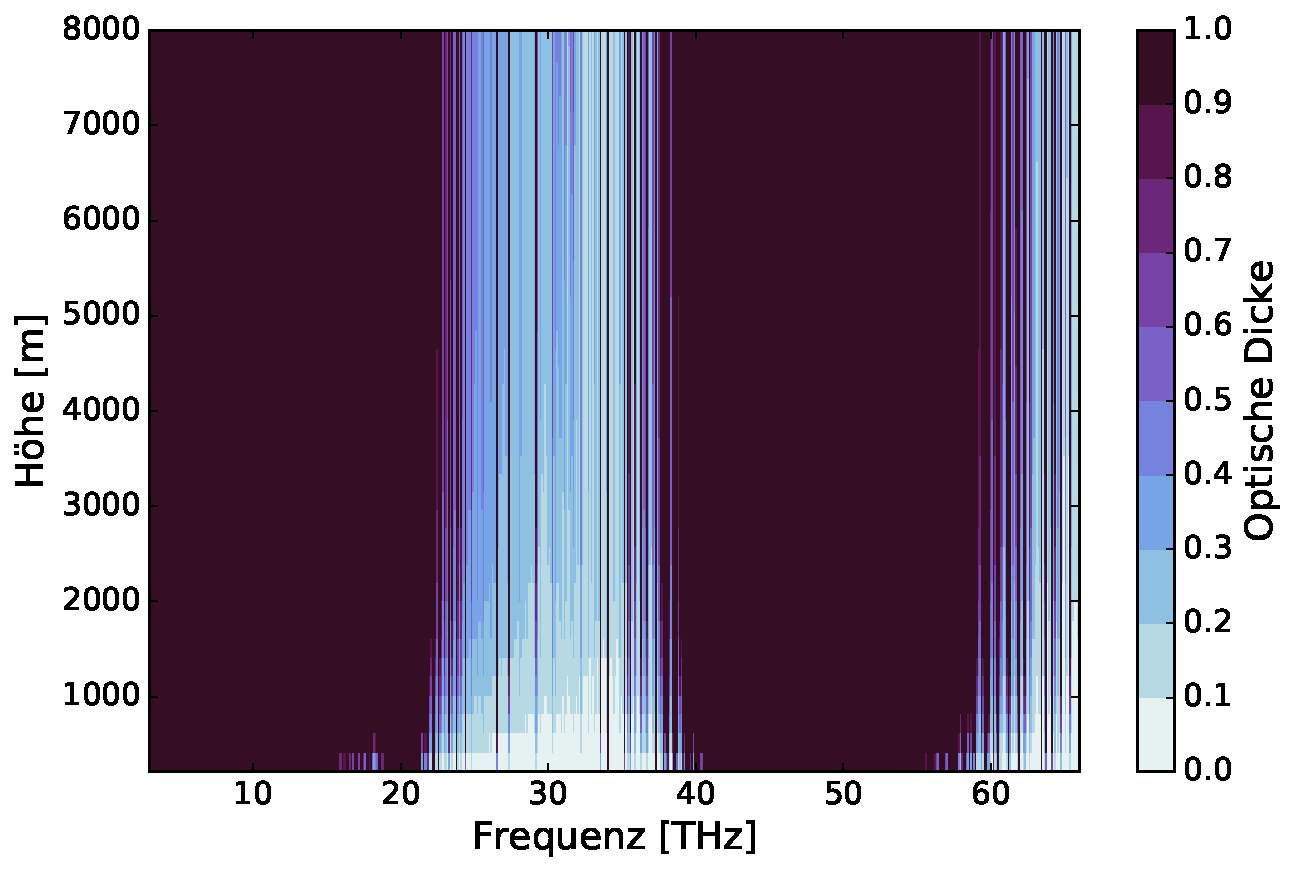
\includegraphics[width=0.5\textwidth]{figures/midlatitude-summer_window.pdf}
  \caption{Höhenabhängigkeit der optischen Dicke für verschiedene Frequenzen.}
  \label{fig:lwr_window}
\end{figure}

Werden zusätzlich Wolken berücksichtigt, verändert sich das Bild drastisch. Die 
optisch durchlässigen Kanäle sind durch die zusätzliche Absorption und Streuung 
der Wolkenteilchen nun nicht mehr durchlässig, sodass die Wolkenbasis die 
maximale Sichthöhe darstellt. Je tiefer sich diese befindet, desto höher ist die 
gemessene Einstrahlung im Fensterbereich. Diese Aussage beruht auf der 
(realistischen) Annahme, dass tiefe Bewölkung wärmer ist als hohe. In der 
Theorie lässt sich somit über die Differenz der langwelligen Einstrahlung 
(Integral über das gemessene Spektrum) und der möglichen Einstrahlung bei 
bodennaher Temperature (Integral über die Planckkurve) das Signal der 
Wolkenunterkante $\Delta L$ ermitteln.
\begin{equation}\label{eq:delta_t}
  \Delta L = L - \int B_\nu(\nu, T_s)\,\partial\nu
\end{equation}
Mit Hilfe der Planckgleichung kann dies in eine Information darüber umgerechnet 
werden, um wie viel Kelvin die Einstrahlung im Kanalbereich kälter ist, als die 
aus den bodennahen Schichten. Unter Annahme eines linearen Temperaturgradienten 
$\gamma$ kann eine Abschätzung der Wolkenbasishöhe erfolgen.
\begin{equation}\label{eq:clb}
  CLB = \frac{\Delta T}{\gamma}
\end{equation}

\subsection{Ergebnisse}\label{subsec:clb_ergebnisse}

\begin{figure*}[ht]
  \centering
  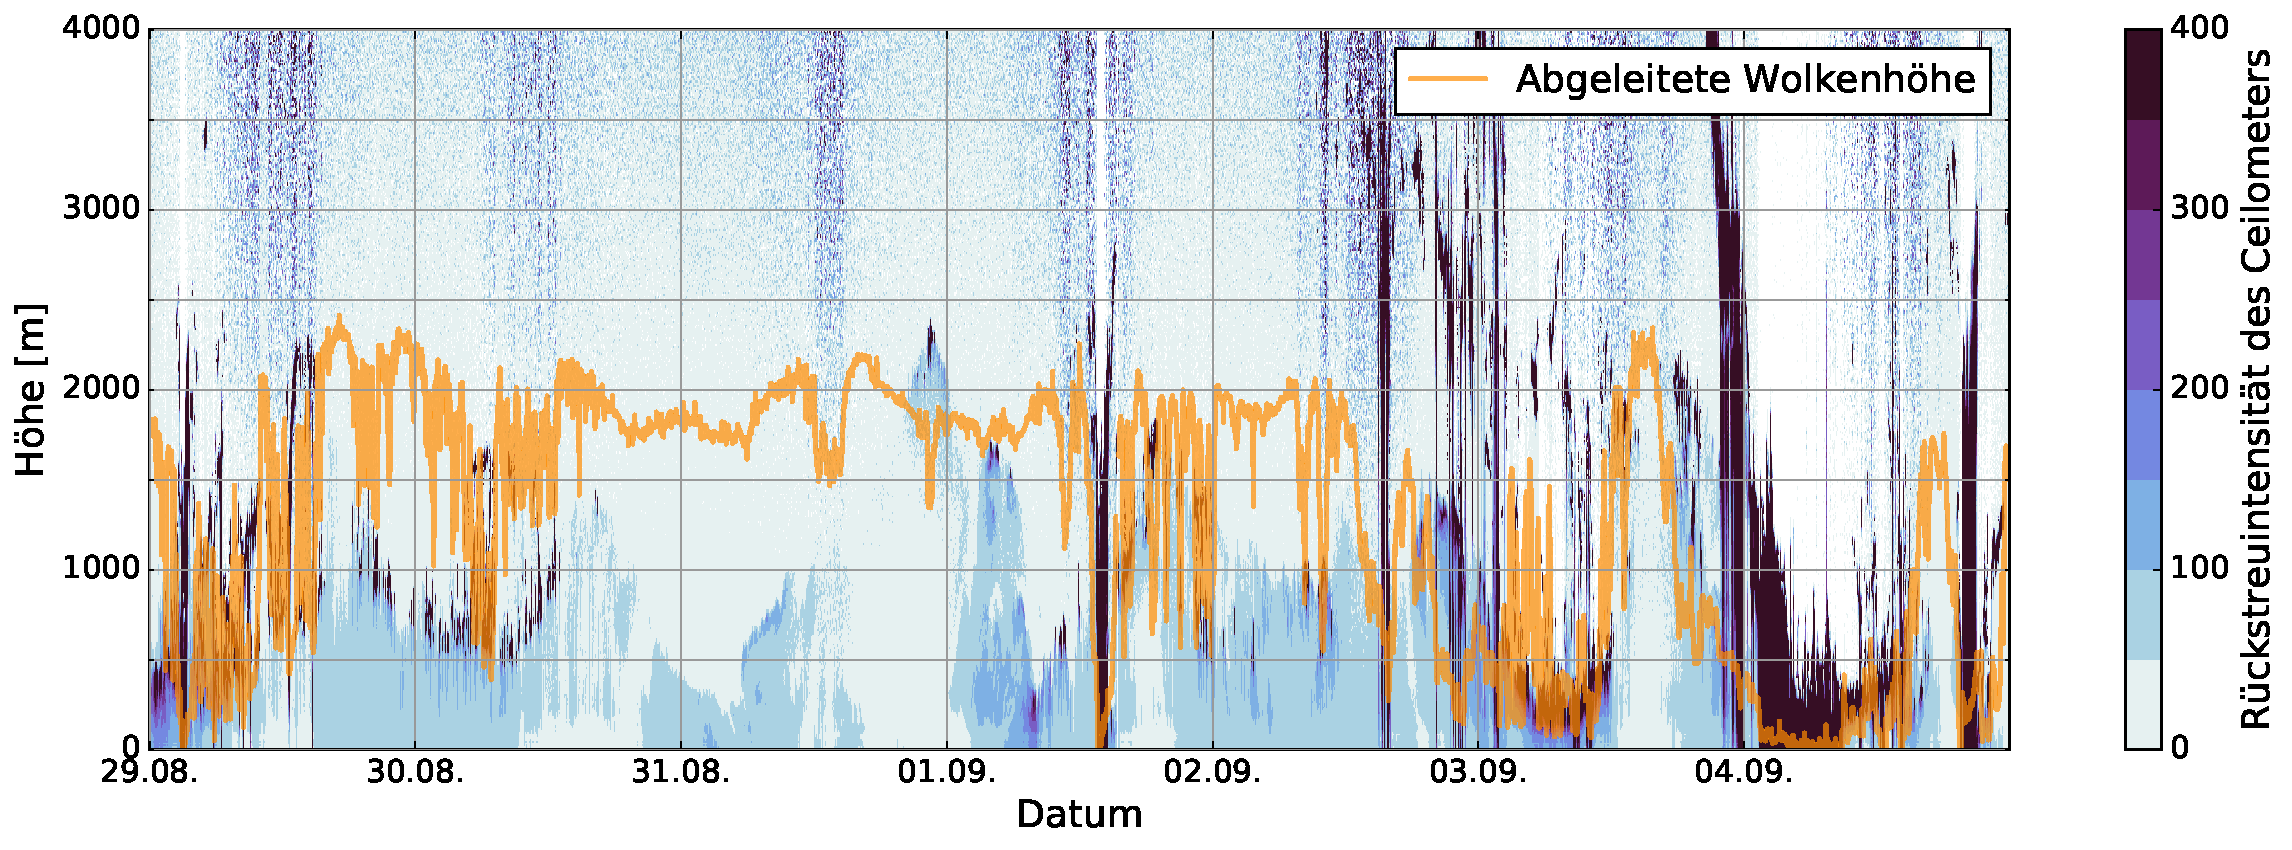
\includegraphics[width=\textwidth]{figures/clb.pdf}
  \caption{Zeitreihe der abgeleiteten Wolkenhöhe (orange) gegen das
  Rückstreuprofil des Ceilometers.}
  \label{fig:clb_zeitreihe}
\end{figure*}

Allgemein muss vorweg erwähnt werden, dass die Messperiode von einem stärkeren
Hochdruckeinfluss beherrscht wurde, die wenig Regen zur Folge hatte. Der
Zeitraum war dementsprechend von Strahlungstagen bzw.\ auch  Tagen mit
teilweise leichterer, aufgelockerter mittelhoher Bewölkung und Zirrusbewölkung
dominiert.  Perioden mit geschlossener, tiefer Stratusbewölkung hatten sich
lediglich spärlich ereignet. Die Analyse der Wolkenunterkantenhöhen ist
entsprechend auf einige wenige Tage und Ereignisse beschränkt.
Nichtsdestotrotz wird der Zeitraum vom 29. August bis 4. September als
Fallbeispiel herangezogen, um das Verfahren der  Wolkenhöhenbestimmung zu
bewerten. Abbildung~\ref{fig:clb_zeitreihe} zeigt die ermittelte
Wolkenbasishöhe des Pyrgeometers im Vergleich mit den Messungen des
Ceilometers.  In den Morgenstunden bis zur frühen Nachmittagszeit des 29.
August konnte das Pyrgeometer die Wolkenunterkantenhöhe recht gut erfassen. Man
kann sehen, dass der Verlauf sowie die Größenordnung für Wolken bis zu einer
Höhe von ca. 2000\,m mit dem Ceilometer annähernd konsistent ist. Zusätlich
bekräftigt die erste Tageshälfte des 3. September sowie der gesamte 4.
September die Annahme, dass das Verfahren bei niedriger, geschlossener
Bewölkung plausible Ergebnisse liefert.

Die Grenzen des Verfahren sind jedoch eindeutig, sobald die Wolkenhöhe zunimmt.
Dieses Verhalten kann in der Nacht des 2. Septembers beobachtet werden. Die
zwischenzeitliche Bewölkung über 2000\,m wird vom Pyrgeometer nicht
registriert. Die hohe Bewölkung kann vom aktiven Messverfahren des Ceilometers
problemlos detektiert werden.  Das Signal in der Rückstreuintensität ist
eindeutig zu erkennen. In der Messung des Pyrgeometers hinterlassen diese
Wolken jedoch kein Signal.  Dies kann verschiedene Ursachen haben.  Zum einen
kann das Signal durch die starke Wasserdampfabsorption in der Atmosphäre
so stark gedämpft worden sein, dass es nicht mehr zu detekieren ist.  Zum
anderen misst das Pyrgeometer die Strahlung aus dem gesamten oberen Halbraum.
Hohe Wolken, die direkt über das Messgerät ziehen, hinterlassen in der
Punktmessung des Ceilometers somit ein stärkeres Signal als in der langwelligen
Einstrahlung.

\begin{table}[ht]
  \centering
  \caption{Korrelation zwischen abgeleiteter Wolkenhöhe und Ceilometermessung
  für Wolken in verschiedenen Höhen.}
  \label{tab:korrelation}
  \begin{tabular}{r|c}
  \textbf{Wolkenhöhe} & \textbf{Korrelationskoeffizient} \\\hline
  0-750\,m     &  0.46 \\
  750-1500\,m  & -0.11 \\
  1500-2250\,m &  0.00 \\
  2250-300\,m  & -0.05 \\
  3000-3750\,m &  0.41 \\
  3750-4500\,m & -0.01 \\
  4500-5250\,m &  0.10 \\
  5250-6000\,m &  0.36 \\
  \end{tabular}
\end{table}

Ein Blick auf die Statistik verdeutlicht, dass die ermittelten Wolkenhöhen
insgesamt nur schwach mit den Messungen des Ceilometers korrelieren. Dieser
Fakt wird anhand der Tabelle~\ref{tab:korrelation} belegt, welche den
Korrelationskoeffizienten $r$ für acht verschiedene Höhenintervalle darlegt.
Obwohl auch im Bereich tiefer Bewölkung  (0-750\,m) die Korrelation nicht
besonders hoch ist ($r = 0.46$), wurde hier das  Maximum von $r$ bestimmt. In
diesem Bereich hat das Pyrgeometer also das größte  Leistungspotential der
Wolkenhöhenbestimmung. Die Schichten in größeren Höhen  weisen eine schwächere
Korrelation vor, die auf die zuvor beschriebenen Fehlerquellen zurückzuführen
ist. Im Höhenbereich zwischen 3000-3750\,m und  5250-6000\,m sieht man einen
sprunghaften Anstieg in $r$, hier wird der Verlauf  höherer Wolken
trotz Offset eventuell erkannt. Die Aussagekraft dieser statistischen Werte
ist jedoch als kritisch anzusehen, da Stichproben über lediglich zwölf Tage
vorliegen. Durch die zusätzliche Aufteilung in Höhenintervalle verringert sich
die Datengrundlage für die statistische Auswertung noch weiter. Die Signifikanz
der ermittelten Korrelationskoeffizienten ist somit in Frage zu stellen.

\section{Wasserdampfsäule}\label{sec:wasserdampfsäule}
Simulationen des langwelligen Strahlungsflusses
(Abschnitt~\ref{sec:strahlungstransfer}) haben gezeigt, dass Wasserdampf der
dominante Absorber im langwelligen Frequenzbereich ist
(Abbildung~\ref{fig:opacity}).  In einem zweiten Versuchsteil wurde daher
untersucht, ob sich durch Messung der langwelligen Einstrahlung der
Wasserdampfgehalt der Atmosphäre abschätzen lässt.  Hierzu wurde eine
Regression über einen Modelldatensatz angewandt
(Abschnitt~\ref{subsec:iwv_regression}). Die Ergebnisse des Verfahrens sind in
Abschnitt~\ref{subsec:iwv_ergebnisse} beschrieben.

\subsection{Regression}\label{subsec:iwv_regression}
Der intergrierte Wasserdampfgehalt ($IWV$) ist das Integral über die Dichte des
Wasserdampfes in allen Atmosphärenschichten (Gleichung~\ref{eq:iwv}). Der $IWV$
ist eine robuste Kennzahl der absoluten Feuchte einer Luftmasse und schon
deshalb eine relevante Größe in der Meteorologie.
\begin{equation}\label{eq:iwv}
  IWV = \int_0^\infty \rho(z) \, dz
\end{equation}
Zusätzlich ist der $IWV$ eine wichtige Größe im atmosphärischen
Strahlungstransfer, da er die optische Dicke im langwelligen Frequenzbereich
maßgeblich beeinflusst. Um diese Abhängigkeit zu quantifizieren und zu nutzen,
wurden Simulationen des Strahlungsflusses für 25.000 Modellatmosphären
durchgeführt. Dieser als Chevallier \cite{Chevallier2006} Atmosphären bekannte
Datensatz ist eine Sammlung von Profilen auf dem globalen Zirkulationsmodell
des EZMW und bildet ein weites Spektrum möglicher atmosphärischer Zustände ab.
Im Anschluss wurde für jede Atmosphäre sowohl die langwellige Einstrahlung $L$
als auch der $IWV$ berechnet (Gleichungen~\ref{eq:lwr_integral}
und~\ref{eq:iwv}). 

In Abbildung~\ref{fig:iwv_lwr_correlation} sind beide Größen grafisch gegeninander
aufgetragen. Es ist deutlich zu erkennen, dass mit steigendem Wasserdampfgehalt
auch die atmosphärische Rückstrahlung zunimmt. Dies ist eine direkte Folge aus
der stärkeren Emissivität der Atmosphäre. Das Kirchhoffsches Strahlungsgesetz
(Gleichung~\ref{eq:kirchhoff}) besagt, dass für Körper im thermischen
Gleichgewicht, die Emission $\epsilon$ und die Absorption $\alpha$ bei gleicher
Frequenz identisch sind; eine optische dichtere Atmosphäre, strahlt auch besser.
\begin{equation}\label{eq:kirchhoff}
  \alpha_\nu = \epsilon_\nu
\end{equation}

Auch die rechnerische Korrelation ($r = 0.757$) der beiden Größen weist eine
starke Abhängigkeit auf. Ein zusätzlicher Einfluss auf die Einstrahlung,
der nicht durch den Wasserdampf erklärt wird, ist insbesondere die Temperature
der Atmosphäre. Die Streuung der Punktwolke in
Abbildung~\ref{fig:iwv_lwr_correlation} lässt sich vermutlich auf diesen
Umstand zurückführen.

\begin{figure}[ht]
  \centering
  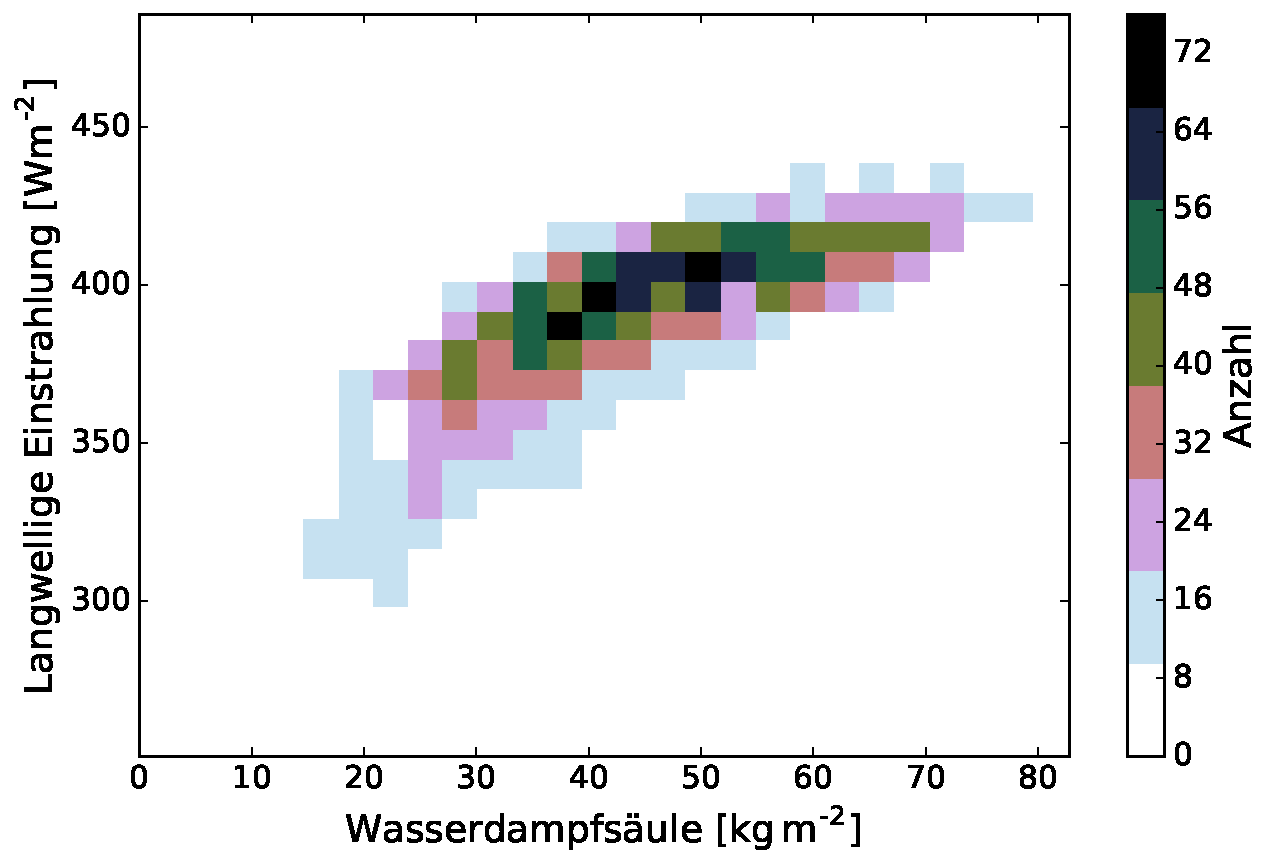
\includegraphics[width=0.5\textwidth]{figures/iwv_lwr_correlation.pdf}
  \caption{Simulierte langwellige Einstrahlung gegen integrierte Wasserdampfsäule
  $IWV$ der Modellatmosphäre.}
  \label{fig:iwv_lwr_correlation}
\end{figure}

Im nächsten Schritt wurde eine Näherungsfunktion aufgestellt
(Gleichung~\ref{eq:iwv_fit}), die eine empirische Bestimmung des $IWV$ auf
Grundlage der langwelligen Einstrahlung so wie einer Reihe Parameter
ermöglicht. Die Werte der Parameter wurden mittels Regression so angepasst,
dass der Verlauf der Funktion den Ergebnissen aus den Simulationen folgt.
\begin{equation}\label{eq:iwv_fit}
  IWV(L,\,a,\,b,\,c) = a \cdot e^{b \cdot L} + c
\end{equation}
Die Form der Funktion ist hierbei grundsätzlich frei wählbar. Es wurden
verschiedene Varianten getestet; Gleichung~\ref{eq:iwv_fit} stellt einen
Kompromiss aus einfacher Form und genügend Freiheitsgraden dar.

\subsection{Ergebnisse}\label{subsec:iwv_ergebnisse}
Mit Hilfe der ermittelten Parameter ist es möglich aus den Messungen der
langwelligen Einstrahlung eine Abschätzung des Wasserdampfgehaltes abzuleiten.
In Abbildung~\ref{fig:iwv_fit_correlation} sind die Resultate der
Näherungsfunktion gegen die Referenzmessungen des Radiometers aufgetragen. Die
Korrelation der beiden Messreihen ($r=0.767$) ist im Rahmen der
Messungenauigkeit identisch mit der Korrelation von $IWV$ und $L$. Diese gute
Übereinstimmung ist auch grafisch am Verlauf der Datenpunkte zu erkennen.
Die Näherung weist jedoch einen deutlichen Offset im Vergleich zur Referenz
auf.  Der Ursprung dieser systematischen Abweichung konnte im Rahmen der
Lehrekursion nicht geklärt werden. Vermutlich wird er jedoch durch die
Vernachlässigung der Temperatur hervorgerufen.

\begin{figure}[ht]
  \centering
  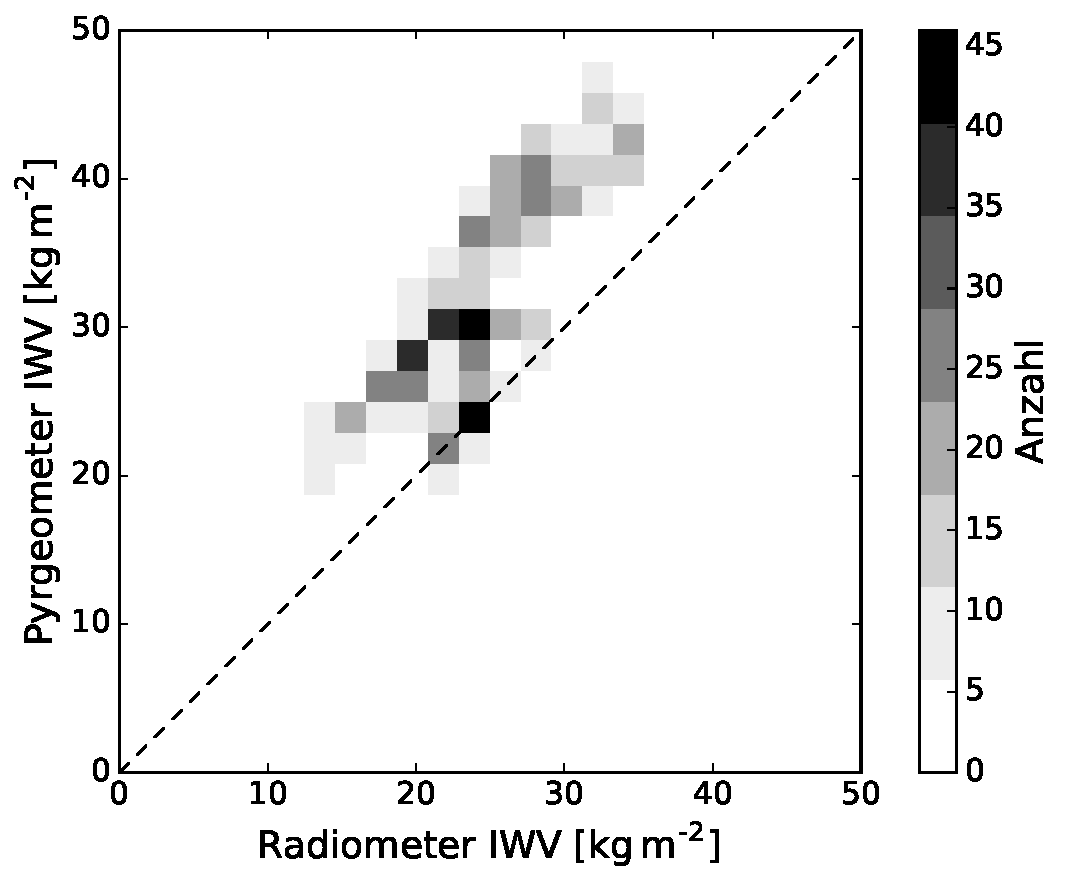
\includegraphics[width=0.5\textwidth]{figures/iwv_fit_correlation.pdf}
  \caption{Integrierte Wasserdampfsäle $IWV$ aus der Regression gegen Messung
  des Radiometers.}
  \label{fig:iwv_fit_correlation}
\end{figure}

\section{Schlussfolgerungen}\label{sec:schlussfolgerungen}
Schlussfolgernd liefern die Untersuchungen jene Erkenntnis, dass sich das 
Pyrgeometer nur bedingt zur Bestimmung der Wolkenhöhe mittels Messung der 
langwelligen Einstrahlung eignet. Die Güte der Ergebnisse ist stark vom 
Parameter der Wolkenhöhe selbst abhängig. Diese Tatsache wurden durch den 
Vergleich mit den Ceilometer-Messungen gezeigt; bei tiefer, geschlossener 
Bewölkung $<$2000\,m ist das angewandte Verfahren ziemlich robust. Die Grenzen 
dieser Methode werden allerdings offensichtlich, sobald die Wolkendecke aufreißt 
und die Wolkenhöhe ansteigt; hier machen sich die drastischen Abweichungen
bemerkbar. Dementsprechend ist diese Methode nur für  stratiforme Bewölkung
präzise, für alle anderen Wolkenfamilien sind die  Ergebnisse ungenau und
nicht zufriedenstellend.

Die Analyse der Wasserdampfsäule hatte zudem zwei Erkenntnisse deutlich gemacht. 
Zum einen wurde festgestellt, dass die Berechnung der Näherungsfunktion mit den 
Referenzmessungen des Mikrowellenradiometers stark korreliert ($r = 0.767$). 
Allerdings ist ein systematischer Fehler zwischen Referenz und Näherung zu
erkennen. Alles in allem  sind die Pyrgeomtermessungen also auch hier trotz
guter Korrelation, aufgrund  des Offsets limitiert. Das Pyrgeometer ist
dementsprechend auch für die  Ermittlung des Wasserdampfgehaltes der Atmosphäre
unzweckmäßig. Zusätzliche Annahmen müssten getroffen werden, die weitere Größen
wie die Temperatur in der Berechnung berücksichtigen, um die Methode robust und
stabil zu machen.

Es kann zusammenfassend gesagt werden, dass Messungen der langwelligen Strahlung 
den zeitlichen Verlauf von Referenzmessungen der Wolkenunterkantenhöhe und der 
Wasserdampfsäule gut wiedergeben können. Die genaueren Zahlenwerte können 
allerdings, je nach Wetterlage und Atmosphärenzustand wenig bis sehr markant 
voneinander abweichen. Aus diesem Grund ist das Potential des Pyrgeometers für 
diese Anwendung eingeschränkt und dem praktischen Einsatz ist eher abzuraten. 

Dieses Experiment hat aufgezeigt, dass ein einfaches Pyrgeometer nicht als 
Alternative empfehlenswert gegenüber den hochmodernen Instrumenten wie dem 
Ceilometer bzw. Mikrowellenradiometer ist. Die hohen Kosten für die Anschaffung 
dieser Geräte wird dann doch tatsächlich durch die Güte und Genauigkeit der 
Messungen, welche mit einer hohen Auflösung abgebildet werden, gerechtfertigt. 

\section{ausblick}\label{sec:ausblick}
Diese Untersuchung hatte lediglich die Parameter Wolkenhöhe und 
Wasserdampfgehalt thematisiert. Gerade bei der Bestimmung der Wolkenhöhe sind
die im Rahmen der Lehrexkursion aufgenommenen Datenreihen deutlich zu kurz, um
die offenen Fragen eindeutig beantworten zu können. Insbesondere 
Wettersituationen mit tiefer Bewölkung waren während des Messzeitraumes sehr selten, sodass eine
genaue statistische Aussage über die Güte des Verfahrens schwierig ist. Ebenso
ist eine genaue Beschreibung der Limitierung des Verfahrens schwierig. Längere
Zeitreihen würden es ermöglichen die in Abschnitt~\ref{subsec:clb_ergebnisse}
vorgestellte Aufteilung in Höhenintervalle auf ein statistisch solideres 
Fundament
zu stellen.

Bei der Bestimmung der Wasserdampfsäule bleibt die Ursache für den Offset 
zwischen Näherung und Referenz unklar. Eine Berücksichtigung der bodennahen Temperatur
in der verwendeten Näherungsfunktion könnte hier Abhilfe schaffen. Grundsätzlich
könnte eine fundierte Analyse der Abhängigkeiten verschiedener atmosphärischer 
Zustandsgrößen weitere Erkenntnisse liefern, die in die Näherung einfließen 
könnten. 

Die offenen Problemstellung sollten nicht als Abschreckung sondern viel mehr als
Anreiz und Anhaltspunkt für nachfolgende Untersuchungen gesehen werden.
Zukünftige Arbeiten könnten auch weitere atmosphärische Größen untersuchen.
Die Quintessenz der Ergebnisse dieses speziellen Versuches sollte
keinesfalls davor abschrecken, weitere Forschungen vorzunehmen, 
welche die Möglichkeiten einfacher, günstiger Messmethoden zu erforschen. Unter 
Umständen können erfolgsversprechendere Ergebnisse in Erfahrung gebracht werden, 
die hilfreich für die Optimierung von Messinstrumenten sein können. Die 
Messmethoden könnten so ausgeweitet und weiterentwickelt werden, wovon 
Meteorologen und Klimawissenschaftler profitieren würden.


% bibliography
\bibliographystyle{IEEEtranS}
\bibliography{references}

\end{document}
